\documentclass[a4paper,12px]{article}
\usepackage{graphicx}
\usepackage[english]{babel}
\usepackage{fancyhdr}
\usepackage{lastpage}
\usepackage{xifthen}
\usepackage[linesnumberedhidden, titlenotnumbered]{algorithm2e}
\usepackage{lipsum}
\usepackage{hyperref}
\usepackage{array}
\usepackage{tabularx}
\usepackage{caption}
\usepackage{amsfonts}
\usepackage{amsmath}

\usepackage{minted}
\usepackage{listings}
\renewcommand\listingscaption{}

\pagestyle{fancy}
\lhead{
\includegraphics[width=7cm]{logoUvA}}
\rhead{\footnotesize \textsc {Report\\ \opdracht}}
\lfoot
{%
    \footnotesize \studentA
    \ifthenelse{\isundefined{\studentB}}{}{\\ \studentB}
    \ifthenelse{\isundefined{\studentC}}{}{\\ \studentC}
    \ifthenelse{\isundefined{\studentD}}{}{\\ \studentD}
    \ifthenelse{\isundefined{\studentE}}{}{\\ \studentE}
}
\cfoot{}
\rfoot{\small \textsc {Page \thepage\ of \pageref{LastPage}}}
\renewcommand{\footrulewidth}{0.5pt}

\fancypagestyle{firststyle}
{%
    \fancyhf{}
    \renewcommand{\headrulewidth}{0pt}
    \chead{
\includegraphics[width=7cm]{logoUvA}}
    \rfoot{\small \textsc {Page \thepage\ of \pageref{LastPage}}}
}

\setlength{\topmargin}{-0.3in}
\setlength{\textheight}{630pt}
\setlength{\headsep}{40pt}

% =================================== DOC INFO ===================================

\newcommand{\titel}{Algorithms and Complexity}
\newcommand{\opdracht}{Week 2: Assignments}
\newcommand{\docent}{Dr. Leen Torenvliet}
\newcommand{\cursus}{Algorithms and Complexity}
\newcommand{\vakcode}{5062ALCO6Y}
\newcommand{\datum}{\today}
\newcommand{\studentA}{Robin Klusman}
\newcommand{\uvanetidA}{10675671}
\newcommand{\studentB}{Maico Timmerman}
\newcommand{\uvanetidB}{10542590}
\newcommand{\studentC}{Boudewijn Braams}
\newcommand{\uvanetidC}{10401040}
\newcommand{\studentD}{Govert Verkes}
\newcommand{\uvanetidD}{10211748}
%\newcommand{\studentE}{Naam student 5}
\newcommand{\uvanetidE}{UvAnetID student 5}

% ===================================  ===================================

\begin{document}
\thispagestyle{firststyle}
\begin{center}
    \textsc{\Large \opdracht}\\[0.2cm]
    \rule{\linewidth}{0.5pt} \\[0.4cm]
    {\huge \bfseries \titel}
    \rule{\linewidth}{0.5pt} \\[0.2cm]
    {\large \datum  \\[0.4cm]}

    \begin{minipage}{0.4\textwidth}
        \begin{flushleft}
            \emph{Supervisor:} \\
            \docent \\[0.2cm]
            \emph{Student:}\\
            {\studentA \\ {\small \uvanetidA \\[0.2cm]}}
            \ifthenelse{\isundefined{\studentB}}{}{\studentB \\ {\small \uvanetidB \\[0.2cm]}}
        \end{flushleft}
    \end{minipage}
    ~%
    \begin{minipage}{0.4\textwidth}
        \begin{flushright}
            \emph{Course:} \\
            \cursus \\[0.2cm]
            \emph{Student:}\\
            \ifthenelse{\isundefined{\studentC}}{}{\studentC \\ {\small \uvanetidC \\[0.2cm]}}
            \ifthenelse{\isundefined{\studentD}}{}{\studentD \\ {\small \uvanetidD \\[0.2cm]}}
            \ifthenelse{\isundefined{\studentE}}{}{\studentE \\ {\small \uvanetidE \\ [0.2cm]}}
        \end{flushright}
    \end{minipage}\\[1 cm]
\end{center}


% =================================== CONTENTS ===================================

\tableofcontents
\clearpage

% =================================== MAIN TEXT ===================================

\section{Flow network}
\subsection{Ford–Fulkerson}

Using the Ford-Fulkerson algorithm we found the maximum flow from source $s$ to
sink $t$. Using Depth First Search paths are found that can increase the maximum
flow. In the following pictures every step of the algorithm is displayed.

\begin{figure}[H]
    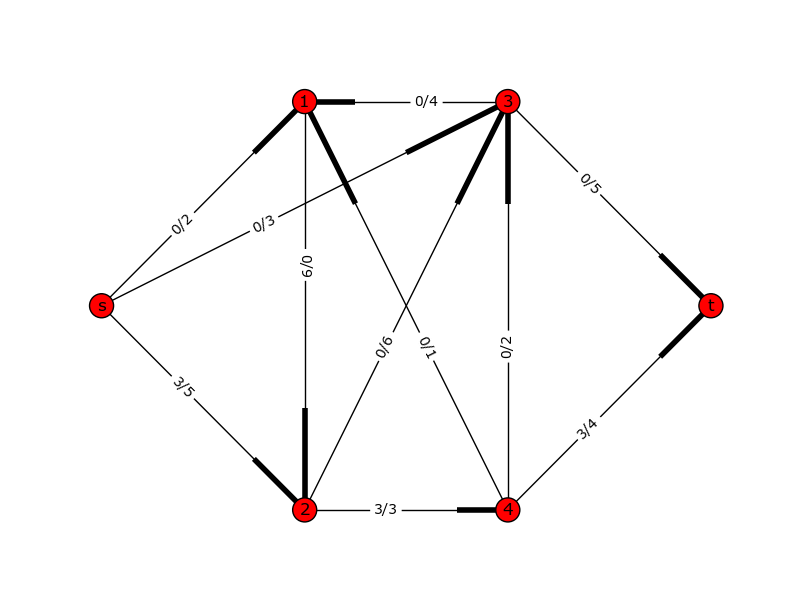
\includegraphics[width=0.8\textwidth]{figure1a_a.png}
    \caption{First step of the Ford Fulkerson algorithm.}
\end{figure}
\begin{figure}[H]
    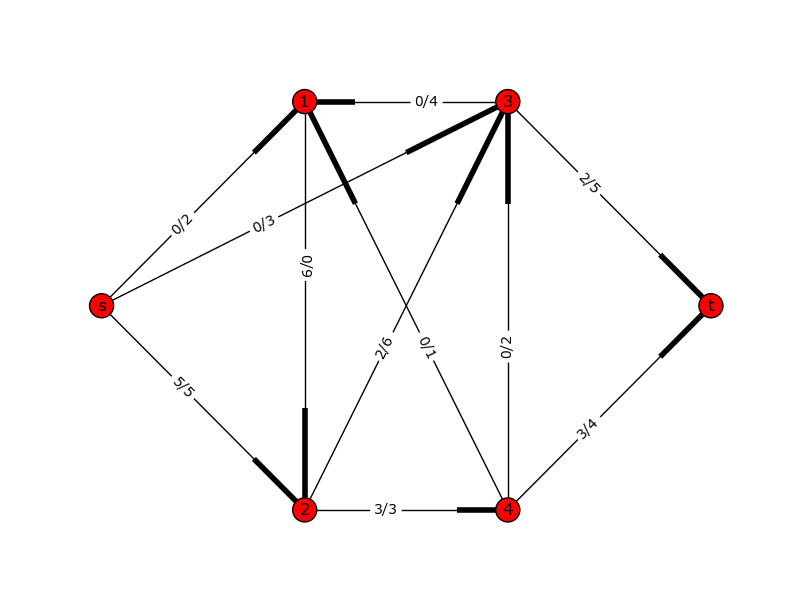
\includegraphics[width=0.8\textwidth]{figure1a_b.png}
    \caption{Second step of the Ford Fulkerson algorithm.}
\end{figure}
\begin{figure}[H]
    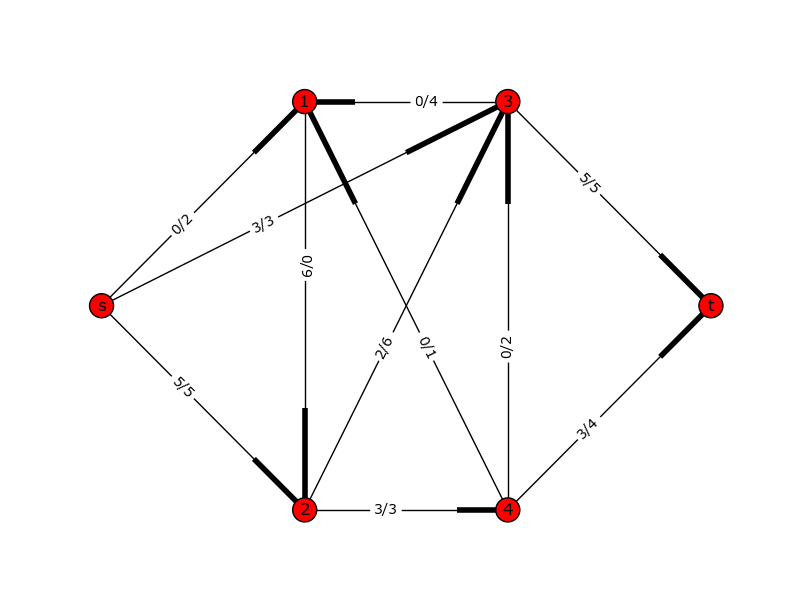
\includegraphics[width=0.8\textwidth]{figure1a_c.png}
    \caption{Final step of the Ford Fulkerson algorithm.}
\end{figure}

\subsection{Layered network}

The picture below describes the layered network with a flow of zero. The flow
blocking path is marked with red.
\begin{figure}[H]
    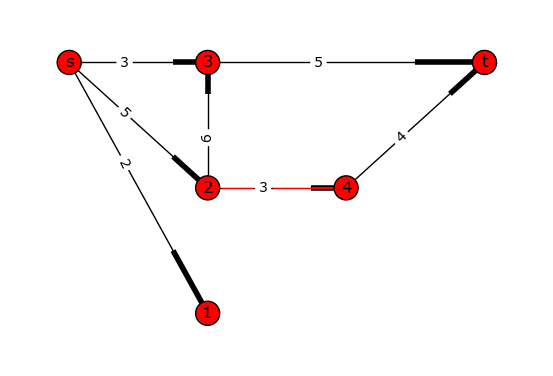
\includegraphics[width=0.8\textwidth]{figure1b_marked.png}
    \caption{Layered network of the graph.}
\end{figure}

\subsection{Cut with minimal capacity}

A cut with minimal capacity is always equal to the maximum flow. As can be seen
in the pictures the maximum flow of the network is equal to 8. So the cut with
the minimum capacity is also equal to 8.

\begin{figure}[H]
    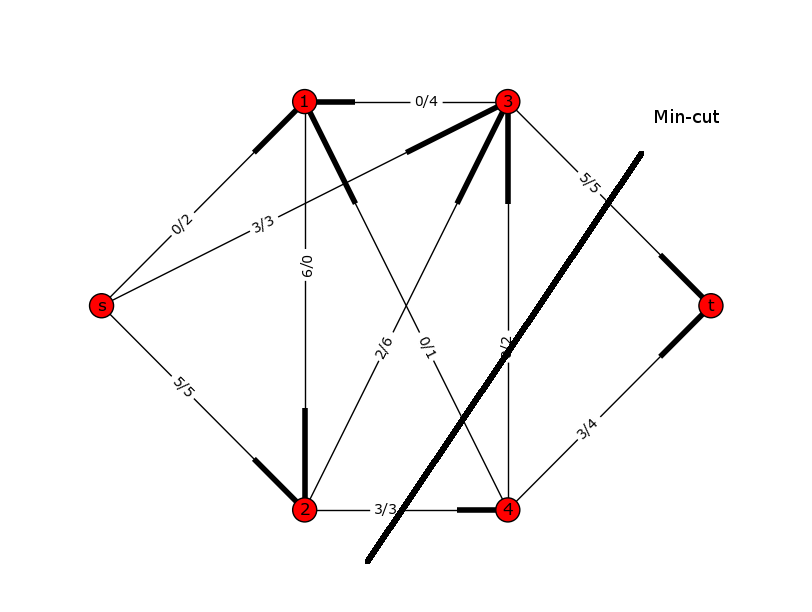
\includegraphics[width=0.8\textwidth]{figure1c.png}
    \caption{Minimum cut in the network.}
\end{figure}

\section{Router}
\section{Router}
\section{Polynomial multiplication}
\subsection{Multiply one-by-one}





% The complexity of this algorithm would be O(n^2 * n!).
% Factorial since all the different permutations of the grandchildren have to be checked each time.
%
% The reason I believe there is no question about the graph of assignment 1 is because this problem is a NP-hard problem and thus rather difficult to implement in an efficient way.
% \begin{listing}
% \inputminted{python}{4.py}
% \caption{Maximum sum path}
% \end{listing}

% =================================== REFERENCES ===================================

%\clearpage
%\bibliographystyle{unsrt}
%\bibliography{bib}

\end{document}
